\chapter{Justification isomorphism}
\label{chap:iso}

In the previous chapter, we introduced the justificatory structure of ontologies and treated the axioms as anonymous \enquote{building blocks} of justifications, without paying consideration to the subexpressions occurring in them. In this chapter, we will go one step further and take into account the logical form of the \emph{axioms} occurring in justifications. 

Given the high expressivity of modern ontology languages, such as OWL, there is the possibility for great diversity in the logical content of ontologies. The fact that many naturally occurring entailments have multiple justifications indicates that ontologies often overdetermine their consequences. However, the multiplicity of justifications might be due mostly to diverse \emph{material}, not \emph{formal}, grounds for an entailment. That is, the logical form of these multiple reasons could be less diverse than their numbers suggest. Such logical similarity indicates that it is possible group justifications into sets of structurally similar ones by the means of an equivalence relation.

A well-known syntactical equivalence relation in OWL is \emph{structural equivalence}. The OWL Structural Specification\footnote{\url{http://www.w3.org/TR/owl2-syntax}} states the condition for two OWL objects (named classes, properties, or instances, complex expressions, or OWL axioms) to be structurally equivalent: in short, it defines the objects to be equivalent if they contain the same names and constructors, regardless of ordering and repetition (in an unordered association). The OWL API implements this notion of structural equivalence by default.

A second equivalence relation is \emph{justification isomorphism}\footnote{Note that, in the spirit of consistent naming, we will use the term \enquote{isomorphism} for the newly introduced equivalent relations despite their not being isomorphisms (i.e. bijective mappings) in the true sense.} which was first introduced in a study of the cognitive complexity of justifications \cite{horridge11gj}: two justifications are isomorphic if they are structurally identical,\footnote{Modulo structural equivalence.} i.e.\ the axioms contain the same \emph{types of} class expressions and only differ in the class, property and instance names. The following example shows two justifications $\J_{1}$ and $\J_{2}$ which we consider to be isomorphic:


\begin{examp}[Isomorphic justifications]
\begin{align*}
\J_{1} &= \{ A \sqsubseteq B \conj \exists r.C, B \conj \exists r.C \sqsubseteq D\} \models A \sqsubseteq D\\
\J_{2} &= \{ E \sqsubseteq B \conj \exists s.F, B \conj \exists s.F  \sqsubseteq D\} \models E \sqsubseteq D
\end{align*}
\end{examp}

It is straightforward to see that in the above justifications the class \dlcn{A} in $\J_{1}$ can be mapped to \dlcn{E} in $\J_{2}$, the property \dlcn{r} to \dlcn{s}, and the class \dlcn{C} to \dlcn{F} in order to obtain identical justifications.

While justification isomorphism helps to eliminate the effects of diverging class, property, and instance names, we can also identify types of justifications which may be considered to be very similar despite their use of different constructors:

\begin{examp}
\label{ex:subex}
\begin{align*}
\J_{1} &= \{A \sqsubseteq B \conj C, B \conj C \sqsubseteq D \} \models A \sqsubseteq D  \\ 
\J_{2} &= \{ A \sqsubseteq \exists r.C, \exists r.C  \sqsubseteq D\} \models A \sqsubseteq D
\end{align*}
\end{examp}
In this example, the semantics of the complex class expressions $B \conj C$ in $\J_{1}$ and $\exists r.C$ in $\J_{2}$  are not relevant for the respective entailment; their occurrences in the justifications and their entailments can be replaced by freshly generated class names without affecting the entailment relation. Such a substitution, in turn, would make the two justifications isomorphic.

Likewise, justifications of different lengths may be considered similar if their general structure of reasoning is identical:
\begin{examp}
\begin{align*}
\J_{1} &= \{A \sqsubseteq B, B \sqsubseteq C \} \models A \sqsubseteq C  \\ 
\J_{2} &= \{ A \sqsubseteq B, B \sqsubseteq C, C \sqsubseteq D \} \models A \sqsubseteq  D
\end{align*}
\end{examp}

These two justifications clearly require the same form of reasoning from a user which means we may consider them to be structurally similar in some way. Strict isomorphism only applies to justifications which contain the same number of axioms; it does not cover situations like one shown above. However, for the purpose of structuring sets of justifications and analysing the logical diversity of a corpus of justifications, capturing those kinds of similarities illustrated in the above examples would be highly desirable. 

In this chapter, we introduce two new equivalence relations, \emph{subexpression-isomorphism} \sisom and \emph{lemma-isomorphism} \lisom,  between justifications based on the subexpressions of their axioms and axiom subsets, respectively, and show how these equivalence relations can be used to determine the logical diversity of a set of justifications. We present an algorithm to detect such equivalence relations and discuss their practical implementation as part of the framework for analysing the justificatory structure of OWL ontologies.


\section{Isomorphism}

Justification isomorphism was first introduced as a way to reduce sampling bias in a user study to validate a model for the cognitive complexity of OWL justifications \cite{horridge11gj}. When studying the cognitive complexity of justifications, we can assume that ontology users will perceive isomorphic justifications as equally difficult to understand, taking into account some variation caused by the complexity of class names and domain knowledge. The ontology corpus from which the justifications in the complexity study \cite{horridge11gj} were sampled was reduced from 64,800 to 11,600 non-isomorphic justifications, thus eliminating the risk of sampling bias caused by presenting users a series of structurally identical justifications. Recall that a justification \J is always defined with respect to a particular entailment \ent; thus, we will use the notation $(\J, \eta)$ to refer to a justification-entailment pair. Justification isomorphism is defined as follows:

\begin{defn}[Justification isomorphism]
Two justifications ($\J_{1},\eta_{1}$), ($\J_{2},\eta_{2}$) are \emph{isomorphic} (($\J_{1},\eta_{1}$) $\isom$ ($\J_{1},\eta_{1}$)) if there exists a bijective renaming $\phi$ which maps class, property, and instance names in $\J_{1}$ and $\eta_{1}$ to class, property, and instance names in $\J_{2}$ and $ \eta_{2}$, respectively, such that $\phi(\J_{1}) = \J_{2}$ and $\phi(\eta_{1}) = \eta_{2}$. 
\end{defn}
\paragraph{Remarks}
\begin{compactenum}
\item The relation \isom is symmetric, reflexive and transitive, from which it follows that \isom is an equivalence relation and thus partitions a set of justifications. Proofs are omitted as these properties are straightforward to see.
 \item Justification isomorphism preserves the numbers and types of axioms and subexpressions in the justifications:
\begin{compactenum}
\item If $\J_{1} \isom \J_{2}$ then $\left|\J_{1}\right| = \left|\J_{2}\right|$.
\item Since the mapping $\phi$ is bijective, we also have $\J_{1} \isom \J_{2} $ implies that $\left|sig(\J_{1})\right| = \left|sig(\J_{2})\right|$.
\item The sets of logical constructs used in $\J_{1}$ and $\J_{2}$ coincide.
\end{compactenum}
\end{compactenum}

\section{Subexpression-isomorphism}

From the above definition of isomorphism it follows that only justifications which have the same number and types of axioms and subexpressions can be  isomorphic. It is easy to see, however, that justifications can have a similar structure despite their use of different class expressions, as demonstrated in Example \ref{ex:subex}. Furthermore, obfuscating complex expressions which can be substituted by propositional variables reduces superfluous clutter in a justification, thus improving the readability of a justification akin to laconic justifications. This motivates a notion of \emph{subexpression-isomorphism}, an equivalence relation which allows not only the mapping of class names, but also that of complex subexpressions.

The idea of finding similarities between concepts in description logics has been widely explored in the work on \emph{unification} and \emph{matching}, e.g.\ \cite{baader98yt,baader99ai,baader09je}, for the purpose of detecting redundant class descriptions in ontologies. Given two class expressions $C$ and $D$, a \emph{unification problem} $C \equiv^{?} D$ asks whether there exists a \emph{substitution} $\sigma$, that is, a mapping from a set of named classes in $C$ into the set of class expressions in $D$, such that $\sigma(C) \equiv \sigma(D)$. The aim of unification is to find a suitable substitution $\sigma$ which maps atomic classes $C$ to (possibly non-atomic) classes in $D$ such that the two classes are made equivalent. 

While the basic idea behind subexpression-isomorphism is based on unification and matching, the concepts are not directly applicable to the given problem of matching justifications. In our case, the inputs are of different shape from the matching problem: the goal is to unify two sets of axioms and the corresponding entailments, rather than matching a single class expression (a class \emph{pattern}) which contains variables to a class expression. That is, we attempt to identify pairs of possibly complex class expressions that, when replaced with names, result in isomorphic justifications. This means that the substitution mechanism as used in unification is not applicable.

We therefore introduce a \emph{justification template} $\jtemplate$, which functions as the \emph{unifying justification} for the isomorphic justifications and \emph{two} substitutions $\phi_{1}, \phi_{2}$ for use in subexpression-isomorphism. We will use freshly introduced entity names $x_{i}$ for the named classes, properties, and instances in a template \jtemplate. In order for subexpression-isomorphism to be transitive, the justifications will have to fulfil certain side-conditions, which will be used in the proof of Proposition \ref{prop:trans}:
\begin{compactenum}[\bfseries S1]
\item For any $C$ in the range of $\phi{1}$ ($\phi{2}$), $C$ is not equivalent to \thing.
\item For any $C$ in the range of $\phi{1}$ ($\phi{2}$) is satisfiable in a \emph{single} element of some interpretation, that is, there is some $I$ such that $\left|C^{I} \right| = 1$.
\item For any $C_{1}$, $C_{2}$ in the range of $\phi^{ac}_{1}$ ($\phi^{ac}_{2}$, respectively), it must hold that $\sig{C_{1}} \cap \sig{C_{2}} = \emptyset$ and $\sig{C_{i}} \cap \sig{\Theta} = \emptyset$, that is, the expressions in the domain and the range of the mappings must be pairwise signature disjoint.
\end{compactenum}

\begin{defn}[Subexpression-isomorphism]
\label{def:siso}
Two justifications ($\J_{1},\eta_{1}$), \\
($\J_{2},\eta_{2}$) are \emph{s-isomorphic} (($\J_{1},\eta_{1}$) \sisom ($\J_{2},\eta_{2}$)) if there exists a justification \emph{template} ($\jtemplate, \eta$) and two injective substitutions $\phi_{1}, \phi_{2}$ satisfying \textbf{S1} to \textbf{S3}, such that 
\begin{compactenum}
\item $\jtemplate \models \eta$
\item $\phi_{1}(\jtemplate)=\J_{1} $ and $\phi_{2}(\jtemplate) = \J_{2}$
\item $\phi_{1}(\eta)=\eta_{1}$ and $\phi_{2}(\eta)=\eta_{2}$.
\end{compactenum}
The mappings $\phi_{1}$ and $ \phi_{2}$ map class, property, and instance names in the template ($\jtemplate, \eta$) to subexpressions of ($\J_{1}$, $\eta_{1}$) and ($\J_{2}, \eta_{2}$), respectively.
\end{defn}
Note that in order to be s-isomorphic, the justifications may differ in the number of subexpressions. As with strict isomorphism, however, they must have the same number of axioms: $\J_{1} \sisom \J_{2} \rightarrow \left|\J_{1}\right| = \left|\J_{2}\right|$. 

\begin{prop}
\label{prop:siso}
S-isomorphism is a more general case of strict isomorphism: $\J_{1} \isom \J_{2} \rightarrow   \J_{1} \sisom \J_{2} $.
\end{prop}


\begin{proof}
Let $(\J_{1}, \eta_{1}) \isom (\J_{2}, \eta_{2})$ via a mapping $\phi$. Then we can consider a  template $\jtemplate$ to correspond to $\J_{1}$, the mapping $\phi_{1}$ is the identity relation $id$ which maps $\J_{1}$ to itself, and $\phi_{2}$ corresponds to the mapping $\phi$ used for strict isomorphism. Thus $\J_{1} \isom \J_{2}$ then $\J_{1} \sisom \J_{2}$.
\end{proof}


\begin{prop}
\label{prop:trans}
The relation \sisom is reflexive, transitive and symmetric for description logics without nominals up to \dl{SRIQ}.
\end{prop}

\begin{proof} Reflexivity and symmetry of the relation are straightforward to see; therefore we will only prove the transitivity of subexpression-isomorphism for logics not containing nominals.

Let $(\J_{a}, \eta_{a}) \sisom (\J_{b}, \eta_{b}) $ via $\phi^{ab}_{1}, \phi^{ab}_{2}, (\jtemplate_{ab}, \eta_{ab})$ and $(\J_{b}, \eta_{b}) \sisom (\J_{c}, \eta_{c}) $ via $\phi^{bc}_{1}, \phi^{bc}_{2}, (\jtemplate_{bc}, \eta_{bc})$, respectively. We aim to show that given this case it is always possible to construct two mappings $\phi^{ac}_{1}, \phi^{ac}_{2}$ and a template  $(\jtemplate_{ac}, \eta_{ac})$, such that $(\J_{a}, \eta_{a}) \sisom (\J_{c}, \eta_{c}) $ via $\phi^{ac}_{1}, \phi^{ac}_{2}$ and $(\jtemplate_{ac}, \eta_{ac})$, as illustrated in Figure \ref{fig:transitivity}. In what follows, we will first describe the construction of  $(\jtemplate_{ac}, \eta_{ac})$ and $\phi^{ac}_{1}, \phi^{ac}_{2}$. We will then show that the entailment relation $\jtemplate_{ac} \models \eta_{ac}$ holds by describing the steps to extend any model $I_{ac}$ for $\jtemplate_{ac}$ to a model of $\eta_{ac}$ by constructing a model $I_{a}$ of $\J_{a}$ (or $I_{c}$ of $\J_{c}$, respectively)

\begin{figure}
\centering
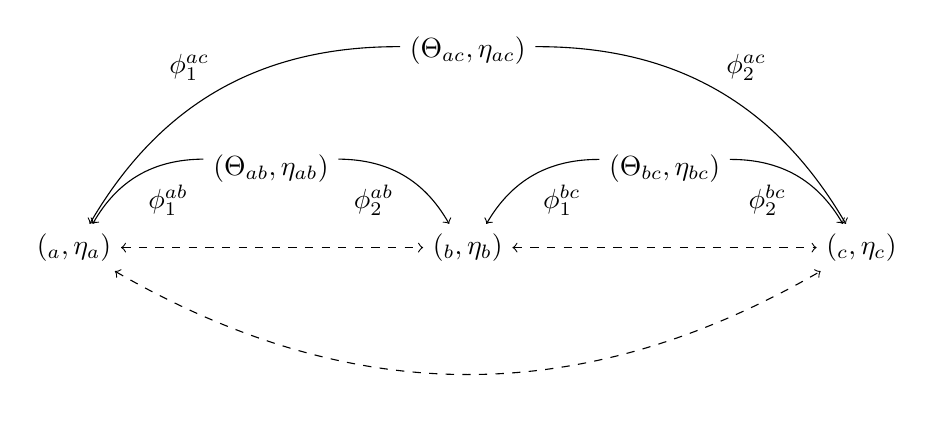
\begin{tikzpicture}
  [scale=1,->,auto=left,every node/.style={draw=none, fill=none}]

  \node (tab) at (3.5,9) {$ (\Theta_{ab}, \eta_{ab})$};
  \node (tbc) at (8.5,9) {$(\Theta_{bc}, \eta_{bc})$};
  \node (tac) at (6,10.5) {$(\Theta_{ac}, \eta_{ac})$};
    
  \node (ja) at (1,8) {$(\J_{a}, \eta_{a})$};
  \node (jb) at (6,8) {$(\J_{b}, \eta_{b}) $};
  \node (jc) at (11,8) {$(\J_{c}, \eta_{c}) $};

  \draw [bend right] (tab) to node {$\phi^{ab}_{1}$} (ja);
  \draw [bend left] (tab) to node [swap] {$\phi^{ab}_{2}$} (jb);
  \draw [ bend right] (tbc) to node {$\phi^{bc}_{1}$} (jb);
  \draw [bend left] (tbc) to node [swap]  {$\phi^{bc}_{2}$} (jc);
  
  \draw [bend right] (tac) to node [swap]  {$\phi^{ac}_{1}$} (ja);
  \draw [bend left] (tac) to node {$\phi^{ac}_{2}$} (jc);


  \draw [<->, dashed] (ja) to node {$\sisom$} (jb);
  \draw [<->, dashed] (jb) to node [swap] {$\sisom$} (jc);
  \draw [<->, dashed, bend right] (ja) to node {$\sisom$} (jc);
    
\end{tikzpicture}
\caption[Three justifications which are s-isomorphic via transitivity.]{Graph representing the relations between three justifications which are subexpression-isomorphic via transitivity.}\label{fig:transitivity}
\end{figure}

First, in order to construct $\Theta_{ac}$ and $\eta_{ac}$, take $\J_{b}, \eta_{b}$ and label each position $p$ in their parse trees\footnote{We use standard notations: $\J|_{p}$ is the subtree/subexpression of \J at position $p$, and $\J[s \rightarrow t]$ the tree obtained by replacing, in \J, the subtree at position $s$ with $t$.} with variables
\begin{compactitem}
\item $(x, ab)$ if $\phi^{ab}_{2}(x) = \J_{b}|_{p}$ and $\jtemplate_{ab}|_{p} = x$
\item $(x, bc)$ if $\phi^{bc}_{1}(x) = \J_{b}|_{p}$ and $\jtemplate_{bc}|_{p} = x$
\end{compactitem}
and the analogue for $\eta_{b}$, i.e.\ we mark nodes in the parse trees of $(\J_{b}, \eta_{b})$ with variables from $(\Theta_{ab}, \eta_{ab})$ if applicable. Please note that a node in the parse trees may be labelled with two such variable labels $(x, ab), (x', bc)$ if $\phi^{ab}_{2}(x) = \phi^{bc}_{1}(x') = \J_{b}|_{p}$.

Now $(\jtemplate_{ac}, \eta_{ac})$ is obtained from this labelled tree by 
\begin{compactitem}
\item removing all subtrees below nodes labelled with variables $(x,\ldots)$ 
\item turning the variables $x$ in these labels $(x,\ldots)$ into leaf nodes (giving precedence to $(x,ab)$ in the presence of two labels), and 
\item serialising the result into a justification and entailment template $(\jtemplate_{ac}, \eta_{ac})$.
\end{compactitem}

We then construct the mappings $\phi^{ac}_{1}$ and $\phi^{ac}_{2}$: if a variable $x$ in $(\jtemplate_{ac}, \eta_{ac})$ originates from a labelling $(x,ab)$ in $\J_{b}$ at position $p$, then 
\begin{compactitem}
\item $\phi^{ac}_{1}(x) = \phi^{ab}_{2}(x)$ and
\item $\phi^{ac}_{2}(x) = \J_{b}|_{p} [t_{j} \rightarrow \phi^{bc}_{2}(y_{j})]$ for $t_{j}$ the positions in $\J_{b}|_{p}$ that are labelled with $(y_{j}, bc)$.
\end{compactitem}
and the analogue for variables originating from labellings $(x, bc)$, and for $\eta_{b}$.

Finally, we need to ensure that the resulting $\jtemplate_{ac}$ indeed entails $\eta_{ac}$. We prove that every model $I_{ac}$ for $\Theta_{ac}$ is a model for $\eta_{ac}$ by first showing that, for $I_{ac}$ a model of $\Theta_{ac}$, we can extend $I_{ac}$ to a model $I_{a}$ for $\J_{a}$ (or the analogue for $I_{c}, \J_{c}$). Given a model $I_{ac} = (\deltaiac, \dotiac)$ of $\jtemplate_{ac}$, we construct $I_{a}$ such that for every $x \mapsto C$ in $\phi^{ac}_{1}$ it holds that $C^{I_{a}} = x^{I_{ac}}$. 

Recall that the expressions in $\J_{a}$ have to fulfil the side conditions \textbf{S1--S3} mentioned above in order for this construction to be possible. The construction steps for $I_{a}$ then are as follows:
\begin{compactitem}
\item Take a model $I_{ac}$ of $\Theta_{ac}$.
\item For each $x \mapsto C$ consider the extension of $x^{I_{ac}} = \{a_{1}, a_{2}, \ldots\}$ where $\left| x^{I_{ac}}\right| = k$ (possibly infinite) and take a model $I$ of $C$ with $\left|C \right| = 1$ to create $k$ \enquote{copies} of $I$. This means we obtain a copy $I_{i}$ of $I$ for each $a_{i} \in x^{I_{ac}}.$
\item For each $a_{i} \in x^{I_{ac}}$, take $I_{i}$ (the $i$-th copy of $I$) and replace the single element $z_{i}$ in $C^{I_{i}}$ with $a_{i}$; in particular, replace $(z_{i}, b) \in r^{I_{i}}$ with $(a_{i}, b)$.
\item Finally, unite the $I_{ac}$ and the models $I_{i}$ created in this way by taking their disjoint union \cite[p 191]{lutz02gy}, that is, the union of the domains and the union of the respective extensions in the models, to obtain a model $I_{a}$ for $\J_{a}$.
\end{compactitem}

With the above steps we have shown that, given any model $I_{ac} \entails \jtemplate_{ac}$, it is possible to construct a model $I_{a}$ such that $I_{a} \models \J_{a}$. Since $\J_{a} \models \eta_{a}$, it also holds that $I_{a} \models \eta_{a}$. 
By construction we know that, for every variable $x$ in $\Theta_{ac}$ or $\eta_{ac}$, it holds that $(\phi^{ac}_{1}(x))^{I_{a}} = x^{I_{ac}}$ and thus $I_{ac} \models \eta_{ac}$. This means that every model $I_{ac}$ for $\Theta_{ac}$ is a model for $\eta_{ac}$, thus the entailment relation $\Theta_{ac} \models \eta_{ac}$ holds. We have therefore shown that we can always construct a template $(\jtemplate_{ac}, \eta_{ac})$ for the justifications $\J_{a}$ and $\J_{c}$, and thus $\J_{a} \sisom \J_{c}$.
\end{proof}

In order to demonstrate the non-transitivity of subexpression-isomorphism in the presence of nominals, we consider a simple counter-example:

\begin{align*}
\O = \{ C \sqsubseteq \{a\},  C \sqsubseteq \{b\}, \{a\} \conj \{b\} \conj \leq 1 r.C \sqsubseteq D\}
\end{align*}
which entails $\eta = C \sqsubseteq D$. The only justification for $\eta$ is the set of all axioms in $\O$. Now modify the ontology to obtain 
\begin{align*}
\O_{a} = &  \{ C \sqsubseteq A,  C \sqsubseteq \{b\}, A \conj \{b\}~ \conj \leq 1 r.C \sqsubseteq D\}\\
\O_{b} = & \{ C \sqsubseteq \{a\},  C \sqsubseteq B, \{a\} \conj B ~\conj \leq 1 r.C \sqsubseteq D\}.\\
\end{align*}
Both $\O_{a}$ and $\O_{b}$ entail $\eta$, and we have that $\O \sisom \O_{a}$ and $\O \sisom \O_{b}$. However, if we substitute the nominals $\{a\}$ and $\{b\}$ with atomic concepts $X$ and $Y$, respectively, in the template
\begin{align*}
 \jtemplate = \{ C \sqsubseteq X,  C \sqsubseteq Y, X \conj Y \conj \leq 1 r.C \sqsubseteq D\}
 \end{align*}
we find that the conjunct $\leq 1 r.C$ is no longer satisfied by all instances of $C$ (and thus $x$ and $y$) and $\jtemplate$ does not entail $C \sqsubseteq D$. This shows that the relation \sisom is not transitive in the presence of nominals.

Finally, note that the substitutions $\phi_{1}$ and $ \phi_{2}$ are injective, but not surjective. As we have shown in the proof of \ref{prop:trans}, injectivity of the mappings is a condition for the transitivity of subexpression-isomorphism. However, the mappings are not surjective, as the set of subexpressions in the justifications  $\J_{1}$ and $\J_{2}$ can be of higher cardinality  than the set of class names in \jtemplate (unless the justifications themselves contain no complex expressions). This is illustrated by the following counter-example of non-surjective mappings: 
\begin{examp}
\begin{align*}
\J_{1} &= \{A \sqsubseteq B, B \sqsubseteq C \}  \\ 
\J_{2}  &= \{ A \sqsubseteq B \conj \exists r.C, B \conj \exists r.C   \sqsubseteq D\}\\
\jtemplate &=  \{x_{1} \sqsubseteq x_{2}, x_{2} \sqsubseteq x_{3} \}  \\ 
\phi_{1} &= \{ x_{1} \mapsto A, x_{2} \mapsto B, x_{3} \mapsto C\}\\
\phi_{2} &= \{ x_{1} \mapsto A, x_{2} \mapsto B \conj \exists r.C, x_{3} \mapsto D\}
\end{align*}
\end{examp}

The set of \emph{all} subexpressions of $\J_{2}$ is $\{A, B, \exists r.C, B \conj \exists r.C, D\}$. $\phi_{2}$ maps only to a subset of these subexpressions; there exists no mapping for the \enquote{smaller} expressions $B$ and $\exists r.C$. This shows that a substitution $\phi$ can be non-surjective.

Despite the mappings being non-surjective, we require each subexpression to either have a corresponding variable in \jtemplate which maps to it directly, or to occur as part of a larger subexpression which has a corresponding variable in \J. This guarantees that the isomorphic justifications have the same number of subexpressions which correspond to variables in \J.


\subsection{Preferred templates}

Given a pair of isomorphic justifications, the template \jtemplate and the substitutions $\phi_{1}, \phi_{2}$ are not necessarily unique; there can be multiple possible substitutions, as demonstrated in Example \ref{ex:preferredsubs}. The substitutions differ in the level of \emph{granularity}, that is, how large a subexpression a variable in \jtemplate is mapped to. Keeping in mind our eventual goal of helping users cope with justifications, we introduce \emph{preferred templates} which reduce the amount of unnecessary detail in a justification template as far as possible. This means that a preferred template $\Theta_{p}$ contains the smallest possible expressions, i.e.\ atomic variable names, where possible. In turn, a substitution $\phi_{i}$ maps a variable in a preferred $\jtemplate_{p}$ to the largest possible subexpression in its corresponding justification $\J_{i}$. Assuming that $\jtemplate, \jtemplate_{p}$ are valid templates for a pair of justifications $(\J_{1}, \eta_{1})$ $(\J_{2}, \eta_{2})$, and $sig(\Theta) \cup sig(\eta)$ is the set of all variables occurring in a template $(\jtemplate, \eta)$, we can define preferred templates as follows:
\begin{defn}[Preferred template]
A template $(\Theta_{p}, \eta_{p})$ is a \emph{preferred template} if there is no template $(\jtemplate, \eta)$ such that $(sig(\jtemplate) \cup sig(\eta)) \subset (sig(\jtemplate_{p}) \cup sig(\eta_{p}))$.
\end{defn}

We illustrate the concept of preferred templates with the following example:
\begin{examp}
\begin{align*}
\J_{1}  &= \{A \sqsubseteq B \conj C\conj D, B\conj C\conj D \sqsubseteq E \}  \\ 
\J_{2}  &=  \{ A \sqsubseteq B \conj \exists r.C, B \conj \exists r.C   \sqsubseteq D\}\\
\jtemplate  &=  \{x_{1} \sqsubseteq x_{2} \conj x_{3}, x_{2} \conj x_{3}\sqsubseteq x_{4} \}  \\ 
\phi_{1}  &=  \{ x_{1} \mapsto A, x_{2} \mapsto B, x_{3} \mapsto C \conj D, x_{4} \mapsto E\}\\
\phi_{2}  &= \{ x_{1} \mapsto A, x_{2} \mapsto B, x_{3} \mapsto \exists r.C, x_{4} \mapsto D\}
\end{align*}\label{ex:preferredsubs}
\end{examp}
In the above example, the template \jtemplate contains a conjunction $x_{2} \conj x_{3}$, which means that only parts of the conjunctions in the justifications $\J_{1}$ and $\J_{2}$ are substituted by variables. It is straightforward to see, however, that there exists an alternative $\jtemplate_{p}$ and substitutions $\phi_{1}'$, $\phi_{2}'$ which substitute larger expressions in the two justifications:

\begin{examp}
\begin{align*}
\jtemplate_{p}   &=  \{x_{1} \sqsubseteq x_{2}, x_{2} \sqsubseteq x_{3} \}  \\ 
\phi_{1}'  &=  \{ x_{1} \mapsto A, x_{2} \mapsto B\conj C\conj D, x_{3} \mapsto E\}\\
\phi_{2}'  &= \{ x_{1} \mapsto A, x_{2} \mapsto B \conj \exists r.C, x_{3} \mapsto D\}
\end{align*}\label{ex:preferred}
\end{examp}
The template $\jtemplate_{p}$ in Example \ref{ex:preferred} has a smaller signature size than $\jtemplate$; it is therefore the preferred template for this pair of justifications. 

%%%%%%%%%%%%%%%%%%%%%%%%%%%%%%%%%%%%%%%%%%

\section{Lemma-isomorphism}

While s-isomorphism covers a number of justifications that can be regarded as equivalent due to them requiring the same type of reasoning to reach the entailment, it only applies to justifications which have the same number of axioms. S-isomorphism does not take into account cases where the justifications differ only marginally in some subset, but where the general reasoning may be regarded as similar nonetheless. We therefore introduce the notion of \emph{lemma-isomorphism}, which extends subexpression-isomorphism with the substitution of subsets of justifications through intermediate entailments, so-called \emph{lemmas}. The general motivation behind lemma-isomorphism is demonstrated by the following example:
\begin{examp}
\begin{align*}
\J_{1} &=  \{ A \sqsubseteq B, B \sqsubseteq C\} \models A \sqsubseteq C\\ 
\J_{2} &= \{ A \sqsubseteq B, B \sqsubseteq C, C \sqsubseteq D \}  \models A \sqsubseteq D
\end{align*}
\end{examp}
It is straightforward to see that both $\J_{1}$ and $\J_{2}$ require the same type of reasoning from a human user. As the justifications only differ in the length of the atomic subsumption chains that lead to the entailment, we can certainly consider them to be \emph{similar} with respect to \emph{some} similarity measure. However, the two justifications are not considered isomorphic with respect to the definitions for strict isomorphism or subexpression-isomorphism. We therefore introduce a new type of isomorphism which takes into account the fact that subsets of justifications can be replaced with intermediate entailments which follow from them. 

A lemma $\lambda$ for a justification \J is an entailment of a subset $S$ of \J. In order to define lemma-isomorphism, we need to introduce two more concepts: \emph{tidy} axiom sets, and justification \emph{lemmatisations}, that is, justifications which are \emph{enriched} with lemmas, as defined by Horridge  \cite{horridge11ab}. 

Tidy axiom sets prevent meaningless lemmatisations by ensuring that the set $S$ that generates a lemma is consistent and does not entail synonyms for \thing or \nothing. They are defined as follows \cite[p 252]{horridge11ab}:
\begin{defn}[Tidy axiom sets]
A set of axioms $S$ is \emph{tidy} if $S \notentails \thing \subcls \nothing$, $S \notentails A \subcls \nothing$ and $S \notentails \thing \subcls A$ for all $A \in \sig{S}$.
\end{defn}
The following definition of \emph{summarising lemmatisations} is based on the definition of lemmatisations given by Horridge \cite[p 253]{horridge11ab}, however, with some modifications: first, Horridge's definition considers the \emph{cognitive complexity} of a lemmatisation in order to ensure that a lemmatisation is \emph{easier} to understand than the justification it is based on. As the complexity of a lemmatisation is not relevant for lemma-isomorphism, we drop this condition. Second, the original definition is too weak for use in lemma-isomorphism, as we will show with an example below; thus, we introduce a new condition for the justification subset $S$ which ensures that the lemmas used for the lemmatisation are \emph{summarising}. And finally, we simplify the definition to omit some unneeded details:
\begin{defn}[Summarising lemmatisation]
Let \justeta be a justification, let $S = \bigcup S_{i}$ be a set of \emph{tidy} subsets of \J, and let $\Lambda_{S} = \bigcup \lambda_{i}$ be a set of lemmas such that $S_{i} \models \lambda_{i}$. The set $\lemmaj = (\J \setminus S) \cup \Lambda_{S}$ is called a \emph{summarising lemmatisation} of \J if 
\begin{compactenum}
\item \lemmaj is a justification for $\eta$,
\item $S_{i}$ are pairwise disjoint.
\end{compactenum}
\end{defn}

If clear from the context, a summarising lemmatisation \lemmaj may also be called a \emph{lemmatised justification}.
\begin{prop}
Given a $S_{i} \in S$ that is substituted with a lemma $\lambda_{i}$ in a summarising lemmatisation \lemmaj, there is no set $S' \subset S_{i}$ such that $S' \entails \lambda_{i}$.
\end{prop}
\begin{proof}
This proposition follows from the minimality condition for justifications: given a justification \justeta, we remove a subset $S_{i} \subseteq\J$ and replace it with a lemma $\lambda_{i}$ such that $(\J \setminus S_{i}) \cup \{\lambda_{i} \}$ is a justification for $\eta$. If there exists a subset $S' \subset S_{i}$ such that $S' \models \lambda_{i}$, then it also holds that $(\J \setminus S_{i}) \cup S' \models \eta $. Therefore, the axioms $S_{i} \setminus S'$ are redundant with respect to the entailment $\eta$, which violates the minimality condition for \lemmaj.
\end{proof}

Given the definitions for lemmatisations, we can now define lemma-isomorphism as an extension to subexpression-isomorphism:
\begin{defn}[Lemma-isomorphism]
Two justifications ($\J_{1},\eta_{1}$), ($\J_{2} ,\eta_{2}$)  are \emph{$\ell$-isomorphic}  (($\J_{1},\eta)$ \lisom $(\J_{2},\eta$)) if there exist \emph{summarising} lemmatisations $\J_{1}^{\Lambda_{S1}}$, $\J_{2}^{\Lambda_{S2}}$ which are s-isomorphic: $\J_{1}^{\Lambda_{S1}} \sisom \J_{2}^{\Lambda_{S2}} $. 
\end{defn}

Lemma-isomorphism as defined above carries two undesirable properties: first, the lemmatised justifications might differ strongly from the original justifications; in the most extreme case, the lemmatisation of a justification can be the entailment itself. We therefore have to introduce a constraint that ensures that lemmatisation must be understandable to a user; thus, we only permit lemmatisations which are based on \emph{obvious} steps, as described in the next section.

Second, we cannot guarantee that lemma-isomorphism using arbitrary lemmas is in fact transitive. Hence, together with the \emph{obviousness} of the lemmas, there are several design decisions to be made when choosing legitimate lemmatisations:

\begin{compactenum}
\item Allow arbitrary non-summarising lemmas.
\item Allow only summarising lemmas. While we cannot show that this preserves transitivity, substituting complete subsets with their lemmas seems more adequate for making lemmatisations easily understandable. 
\item Allow only specific types of lemmas, e.g.\ entailments of atomic subsumption chains. We take this approach below in order to restrict lemmatisations to obvious proof steps.
\item Allow only specific types of atomic subsumption chains, e.g.\ \emph{maximal} atomic subsumption chains. As we will show in Section \ref{sec:subschains}, this is necessary for a practical implementation of lemma-isomorphism.
\end{compactenum}

We will first discuss the issue of obvious steps for lemmatisations, before selecting a suitable type of lemmas---entailments of atomic subsumption chains---which are both cognitively adequate and can be computed in practical time.


\subsection{Lemmatisations and obvious steps}
\label{sec:obvious} 

The notion of \emph{obvious logical inferences} \cite{davis81sz} describes how proof steps which are \emph{obvious} for a reader can be omitted without losing information that may be important for understanding the proof. We adapt this notion of obvious steps in order to allow only lemmatisations which are easily understandable for a human reader, that is, lemmas which follow from a subset of a justification in a straightforward fashion.

While research on human understanding of description logic is fairly limited, the works by Horridge \cite{horridge11gj} and Nguyen \cite{nguyen12ab} provide us with two different models for determining the complexity of justifications and justification subsets, respectively, and thus the obviousness of lemmas.

%The complexity model proposed by Horridge et al.\ \cite{horridge11gj} is based on an exploratory study which identified properties of justifications that can be considered hard to understand for users. These properties include, amongst others, the number of different axiom types and class constructors in the justification and the entailment, whether a justification axiom contains certain constructs (e.g.\ a universal implication on the LHS of a subsumption axiom), and the maximum modal depth of the expressions in the justification. Given a justification and entailment, the model generates a value between 0 (very easy) and roughly 2000 (very hard) to predict the difficulty a user will have in understanding the justification. In an evaluation study, the model was shown to be accurate for a number of justifications, while it failed to predict the difficulty users would have with non-laconic justifications.

%Nguyen et al.\ \cite{nguyen12ab} propose a purely empirical model which predicts the complexity of frequently occurring patterns, or \emph{rules}, in justifications. These rules, consisting of between 1 and 4 axioms, were translated into natural language and presented to a large number of test subjects using a Mechanical Turk platform. Based on the performance of the test subjects on confirming whether a statement followed from a rule, the rules were ranked in order of difficulty. The 57 rules that were identified and ranked in this process cover approximately 48\% of the entire test corpus of 30,000 justifications used in the study.

While the rankings determined by Nguyen et al.\ \cite{nguyen12ab} seem to cover the most frequently occurring justification subset patterns, they do not include atomic subsumption chains, which have been found to be one of the most prevalent and easiest recognizable patterns \cite{horridge11gj}. We therefore focus on atomic subsumption chains for the purpose of demonstrating the effects of lemma-isomorphism.


\subsubsection{Atomic subsumption chains}
\label{sec:subschains}

Given an atomic subsumption chain of the type $S = \{A_{0}\sqsubseteq A_{1}, A_{1} \sqsubseteq A_{2} \ldots A_{n-1} \sqsubseteq A_{n}\}$ in a justification, often only the relation between the subclass $A_{0}$ in the first axiom and the superclass $A_{n}$ in the last axiom is relevant for understanding the how the chain contributes to the justification. That is, the subsumption chain produces a summarising lemma $A_{0} \subcls A_{n}$ which is the only piece of information required for the justification. The step from the subclass to the final superclass was found to be \emph{obvious} for OWL users who were presented with justifications containing ordered and indented subsumption chains of this type \cite{horridge11gj}. Therefore, a suitable lemmatisation of a justification containing an atomic subsumption chain is the justification obtained by substituting the chain with its conclusion in the form of a single axiom $A_{0} \sqsubseteq A_{n}$.


\paragraph{Maximal atomic subsumption chains}

Recall that we require the lemmatisations of atomic subsumption chains in a justification to be summarising, that is, the subsumption chain can be substituted by a single axiom and the entailment of the justification still holds. However, axioms that appear to be a single atomic subsumption chains may not always be such a \emph{maximal} chain: if a chain $A_{0} \subcls \ldots \subcls A_{n} $ can be substituted by a summarising lemma $\lambda$, and there exists a longer chain $A_{0} \subcls \ldots \subcls A_{n+1}$, then the longer chain cannot always be substituted by a summarising lemma $\lambda'$. It is certainly possible for a set of axioms to form an apparently maximal subsumption chain in which only a subset of the chain can be substituted by a summarising lemma, as shown in the following example: 
\begin{examp}
\label{ex:non-max-subschain}
\begin{align*}
\J = & \{A \subcls \exists r.C, A \sqsubseteq B, B \sqsubseteq C, C \sqsubseteq D, C \conj \exists r.D \sqsubseteq E \} \models A \sqsubseteq E
\end{align*}
\end{examp}

Take the justification \J in Example \ref{ex:non-max-subschain}. The axiom set $\{A \sqsubseteq B, B \sqsubseteq C, C \sqsubseteq D\}$ is a maximal atomic subsumption chain in \J which can be substituted by its entailment \dlax{A \subcls D}. It is clear to see, however, that the entailment does not hold in this lemmatisation as the important lemmas \dlax{A \subcls C} and \dlax{C \subcls D} would be lost. We can only substitute part of the subsumption chain, namely $\{A \sqsubseteq B, B \sqsubseteq C\}$ with its entailment \dlax{A \subcls C}; we call the axiom set $\{A \sqsubseteq B, B \sqsubseteq C\}$ a non-maximal chain.

Non-maximal subsumption chains are problematic as they can to lead to non-transitivity of lemma-isomorphism, as is shown in the following example:
\begin{examp}
\scriptsize
\begin{alignat*}{3}
\J_{a}  \entails X \subcls Y &\quad\quad& \J_{b}  \entails X \subcls Y &\quad\quad& \J_{c}  \entails X \subcls Y\\
X \subcls (A_{0} \conj A_{2}) \conj (\forall r.A_{0} \conj \forall s.A_{4}) &\quad\quad& X \subcls (B_{0} \conj B_{2}) \conj (\forall r.B_{0} \conj \forall s.B_{4}) &\quad\quad& X \subcls (C_{0} \conj C_{2}) \conj (\forall r.C_{0} \conj \forall s.C_{4}) \\
 (A_{1} \conj A_{5}) \conj (\forall r.A_{3} \conj \forall s.A_{5}) \subcls Y &\quad\quad&  (B_{1} \conj B_{5}) \conj (\forall r.B_{3} \conj \forall s.B_{5}) \subcls Y &\quad\quad&  (C_{1} \conj C_{5}) \conj (\forall r.C_{3} \conj \forall s.C_{5}) \subcls Y \\
 A_{0} \subcls A_{1} && B_{0} \subcls B_{1} && C_{0} \subcls C_{3} \\
 A_{2} \subcls A_{5} && B_{1} \subcls B_{2} && C_{4} \subcls C_{5} \\
 && B_{2} \subcls B_{3} && \\
 && B_{3} \subcls B_{4} && \\ 
 && B_{4} \subcls B_{5} && 
 \end{alignat*}
\end{examp}
In the above example, the three axiom sets are justifications for \dlax{X \subcls Y}. It holds that $\J_{a} \lisom \J_{b}$ and $\J_{b} \lisom \J_{c}$ via lemmatisations $\J_{b}^{\lambda_{1}}$ and $\J_{b}^{\lambda_{2}}$, respectively. While the set of atomic subsumption axioms in $\J_{b}$ appears to be a single maximal chain, it cannot be substituted with a single lemma without breaking the entailment. In $\J_{b}^{\lambda_{1}}$ the atomic subsumption chain $B_{0} \ldots B_{5}$ is substituted with the two lemmas $\lambda_{11} = B_{0} \subcls B_{1}, \lambda_{12} = B_{2} \subcls B_{5}$, which makes the lemmatisation strictly isomorphic to $\J_{a}$. The analogue holds for $\J_{b}^{\lambda_{2}}$ which is strictly isomorphic to $\J_{b}$ via the two lemmas $\lambda_{21} = B_{0} \subcls B_{3}, \lambda_{22} = B_{4} \subcls B_{5}$. However, $\J_{a}$ and $\J_{c}$ are clearly not s-isomorphic. This shows that lemma-isomorphism which allows the substitution of non-maximal chains with lemmas can lead to non-transitivity of the relation. 

While we have not yet proved that maximal-chain lemma-isomorphism is guaranteed to be transitive, restricting the lemmatisations to maximal chains removes one possible cause of non-transitivity. However, the transitivity of lemma-isomorphism with maximal atomic subsumption chains remains an open question; for the time being, we treat all results of the lemma-isomorphism implementation as possible approximations. This means that it is possible that some sets of justifications may be considered to be non-isomorphic when they actually are. Hence, we may potentially over-estimate the logical diversity of a corpus of justifications and under-estimate the effects of lemma-isomorphism, which we consider acceptable for the purpose of demonstrating the concept of lemma-isomorphism.

%It is not clear whether non-maximality of a chain that is substituted by a summarising lemma affects transitivity of lemma-isomorphism; this remains an open question. For now, however, we have another, practical reason for restricting lemma-isomorphism to maximal chains, that is, for excluding chains of the type shown in Example \ref{ex:non-max-subschain}. In an implementation of the atomic subsumption chain lemmatisation, detecting non-maximal chains would would require searching through all subchains of the maximal atomic subsumption chain in order to find a suitable, substitutable, chain. 

%While this is of course not a problem in theory, the search space of this operation would be the powerset of $S$ where $S = \{\alpha_{i}\}$ for $\alpha_{i}$ an axiom of type $A_{i} \subcls A_{i+1}, 0 \leq i \leq n$. This means the number of potential non-maximal chains is $\setcard{\mathcal{P}(S)} = 2^{n}$. Due to the potentially large number of lemmatisation attempts, this behaviour is not practical for an implementation. Our current implementation only attempts to substitute maximal chains, which may lead to false negative results when attempting to compare two justifications which are only lemma-isomorphic through subchain substitution. Since this leads to under-estimating the number of isomorphic justifications, this seems an acceptable trade-off.

In summary, for the purpose of demonstrating lemma-isomorphism in this thesis, we restrict the admissable lemmatisations of a justification (\J, \ent) to 
\begin{compactitem}
\item atomic subsumption chains of type $A_{0} \subcls \ldots \subcls A_{n}$ 
\item that are summarising, i.e.\ $\J \setminus S \cup \{\lambda\} \models \ent$ for $S$ a set of axioms of type $A_{0} \subcls \ldots \subcls A_{n}$ and $\lambda = A_{0} \subcls A_{n}$
\item that are maximal, i.e.\ given a chain $A_{0} \subcls \ldots \subcls A_{n}$, there exists a summarising $\lambda = A_{0} \subcls A_{n}$ such that $\J \setminus S \cup \{\lambda\} \models \ent$.
\end{compactitem}

%We can show transitivity of lemma-isomorphism using summarising, maximal atomic subsumption chains as follows:

%Let us consider three justifications $(\J_{a}, \eta_{a}), (\J_{b}, \eta_{b}), (\J_{c}, \eta_{c})$ such that $(\J_{a}, \eta_{a}) \lisom (\J_{b}, \eta_{b})$ and $(\J_{b}, \eta_{b}) \lisom (\J_{c}, \eta_{c})$. From the definition of lemma-isomorphism it follows that the justifications have summarising lemmatisations $(\J_{a}, \eta_{a})^{\Lambda}, (\J_{b}, \eta_{b})^{\Lambda}, $ and $ (\J_{c}, \eta_{c})^{\Lambda}$ such that $(\J_{a}, \eta_{a})^{\Lambda} \sisom (\J_{b}, \eta_{b})^{\Lambda}$ and $(\J_{b}, \eta_{b})^{\Lambda} \sisom (\J_{c}, \eta_{c})^{\Lambda}$, that is, the lemmatisations are subexpression-isomorphic.

%Since we require the lemmatisations to be summarising, any chain of length $n$ that is substituted can be substituted with a single subsumption axiom; that is, regardless of the length of the chain, we can assume that the lemmatisation contains a single atomic subsumption axiom in place of the chain. The lemmatisations will all contain the same number of axioms, with atomic subsumption axioms in corresponding positions. It is straightforward to see that that if $(\J_{a}, \eta_{a})^{\Lambda} \sisom (\J_{b}, \eta_{b})^{\Lambda}$ and $(\J_{b}, \eta_{b})^{\Lambda} \sisom (\J_{c}, \eta_{c})^{\Lambda}$, then $(\J_{a}, \eta_{a})^{\Lambda}$ will also be subexpression-isomorphic to $(\J_{c}, \eta_{c})^{\Lambda}$. Transitivity then follows from the transitivity of subexpression-isomorphism.


\section{Equivalence and superfluity}

For the purpose of analysing the diversity of reasons why an entailment holds in an ontology, we need to take into account another aspect of justifications, namely the superfluousness of subexpressions in an axiom. Since justifications are sets of axioms \emph{as they are asserted in the ontology}, it is possible for such an axiom to contain parts which are not relevant with respect to the entailment. This can have several possible effects: 1) A justification can contain \emph{multiple} reasons for an entailment to hold. 2) Two justifications can have exactly the same reason why an entailment holds and only differ in their superfluous parts; this results in \emph{fewer} logical reasons than material justifications. 3) A justification can have parts which interact with \emph{other} axioms in the ontology to form entirely \emph{new} justifications. These phenomena are also known as facets of \emph{justification masking} \cite{horridge10bg} which was introduced in Chapter \ref{chap:background}. In order to take into account the effects of masking in justifications and to eliminate potentially distracting superfluous expressions, Horridge et al.\ \cite{horridge08yi} defined \emph{laconic} justifications which we also discussed in Chapter \ref{chap:background}.

It is clear to see that superfluity can lead to justifications being considered non-isomorphic, despite them being identical \enquote{in principle} and requiring the same reasoning strategy. As a simple example, take the following two justifications:
\begin{align*}
\J_{1} = & \{\dlax{A \subcls B \conj C, B \subcls D}\} \models \dlax{A \subcls D}\\
\J_{2} = & \{\dlax{A \subcls B, B \subcls D}\} \models \dlax{A \subcls D}
\end{align*}
Both justifications only require atomic subsumption chain reasoning; the conjunct $C$ in $\J_{1}$ is superfluous as it does not affect the entailment. However, the justifications could not be considered to be isomorphic with respect to any of our relations. Note that the superfluity itself is not the culprit here, since a similarly superfluous conjunct in $J_{2}$ would cause the justifications to be (strictly or subexpression-) isomorphic nonetheless. It is the superfluity (or lack thereof) in different positions which causes the structural similarity of the justifications to be concealed.

We know that non-laconic justifications are highly prevalent in OWL ontologies, as shown by a study of 72 BioPortal ontologies in which over 82\% of the justifications were found to contain superfluous expressions \cite{horridge11ab}. This indicates that in order to obtain a more accurate picture of the logical diversity of a set of justifications we may choose to identify isomorphic justifications based on their laconic versions. Note that due to internal masking, a justification can have \emph{multiple} laconic versions. This means that a necessary condition for the  justifications to be considered isomorphic is that \emph{all} their laconic versions have to be isomorphic.


%%%%%%%%%%%%%%%%%%%%%%%%%%%%%%%%%%%%%%%%%


\section{Implementing an isomorphism checker}

Having introduced the basic notions of isomorphism in the previous section, we will now discuss our approach to implementing an isomorphism checker which covers all three types of isomorphism. We outline the algorithm for detecting isomorphism which is based on a comparison between the parse trees of the justifications to be matched, and discuss some of the basic optimisations that can be applied to improve the performance of the isomorphism checker. Finally, we describe how the j-graph introduced in Chapter 4 can be extended to include justification templates for structurally isomorphic justifications.

\subsection{Algorithm and implementation}

The general idea behind the implementation of a program to check whether two justifications are isomorphic is the comparison of the \emph{parse trees} of the two justifications. Each axiom in a  justification is parsed into its parse tree where the nodes are labelled with either entity names (properties or classes), OWL constructors, or integers (in the case of cardinality restrictions). The parse tree of a justification simply contains each axiom parse tree as child of a blank root node. To simplify the algorithm, the respective entailments are treated \emph{separately} from the justification parse trees, as this allows us to treat every axiom subtree in the justification parse tree equally. An example of a justification parse tree (without the respective parse tree of the entailment) is shown in Figure \ref{fig:parsetree}. 


\begin{figure}
\centering{
\begin{tikzpicture}
  [scale=1,->,auto=left]

\node (root) at (3.5,9) {\J};
  
\node (ax1) at (0,8)  {$\sqsubseteq$};
\node (ax2) at (3.5,8) {$\sqsubseteq$};
\node (ax3) at (7,8)  {$\sqsubseteq$};

\node (ax1lhs) at (-1,7.25)  {$A$};
\node (ax1rhs) at (1,7.25)  {$\exists$};
\node (ax1rhslhs) at (0.5,6.5)  {$r$};
\node (ax1rhsrhs) at (1.5,6.5)  {$B$};

\node (ax2lhs) at (2.5,7.25) {$B$};
\node (ax2rhs) at (4.5,7.25)  {$C$};
 
\node (ax3lhs) at (6,7.25)  {$\exists$};
\node (ax3lhslhs) at (5.5,6.5)  {$r$};
\node (ax3lhsrhs) at (6.5,6.5)  {$C$};
\node (ax3rhs) at (8,7.25)  {$D$};

\draw (root) to node {} (ax1);
\draw (root) to node {} (ax2);
\draw (root) to node {} (ax3);

\draw (ax1) to node {} (ax1lhs);
\draw (ax1) to node {} (ax1rhs);
\draw (ax1rhs) to node {} (ax1rhslhs);
\draw (ax1rhs) to node {} (ax1rhsrhs);

\draw (ax2) to node {} (ax2lhs);
\draw (ax2) to node {} (ax2rhs);
 
\draw (ax3) to node {} (ax3lhs);
\draw (ax3lhs) to node {} (ax3lhslhs);
\draw (ax3lhs) to node {} (ax3lhsrhs);
\draw (ax3) to node {} (ax3rhs);

    
\end{tikzpicture}
\caption[Parse tree of a justification.]{Parse tree of $\J = \{\dlax{A \subcls \exists r.B, B \subcls C, \exists r.C \subcls D}\}$ \entails \dlax{A \subcls D}. }
\label{fig:parsetree}
}
\end{figure}

Given the parse trees of two justifications $(\J_{1}, \eta_{1})$,  $(\J_{2}, \eta_{2})$, the algorithm answers \enquote{true} if the justifications are isomorphic wrt. one of the given definitions for isomorphism, and \enquote{false} otherwise. While there exist algorithms for tree-isomorphism (e.g. \cite{shamir99aa}), we chose to implement a naive matching algorithm, as this would allow us to extend the algorithm from strict to subexpression-isomorphism in a straightforward fashion.

For strict isomorphism, the algorithm answers \enquote{true} if it can construct a mapping $\phi$ (that is, a set of pairs $(n1, n2)$) which maps nodes $n1$ in the parse trees of $\J_{1}$ and $\eta_{1}$ to nodes $n2$ in $\J_{2}$ and $\eta_{2}$ such that $\phi(\J_{1}) = \J_{2}$ and $\phi(\eta_{1}) = \eta_{2}$. For subexpression-isomorphism, we deviate from the given definition and attempt to find only a single mapping $\phi$ which maps subtrees in $\J_{1} $ and $\eta_{1}$ to subtrees in $\J_{2}$ and $\eta_{2}$, respectively. Finally, as lemma-isomorphism is based on subexpression-isomorphism, we first lemmatise the justifications, then apply the algorithm for detecting subexpression-isomorphism to the lemmatised justifications.

An outline of the algorithm for strict isomorphism and its subroutines are given in Algorithms \ref{alg:doom} and \ref{alg:subroutines}, whereby  $\textsc{childCount()}$, $\textsc{removeChild()}$, and $\textsc{getChildAt()}$ can be interpreted as standard operations on a tree structure. The algorithm traverses the parse trees of $\J_{1}$ and $\J_{2}$ (denoted by $e1$ and $e2$ in the pseudocode) depth-first, left to right, and attempts to construct a set $Mappings$ of candidate mappings. It checks at each node whether the nodes at this position in the parse trees are compatible in the context of the current mapping $\phi$. Note that the parse trees of the entailments are not considered here; they only come into play in the final call to $\textsc{isCorrectMapping()}$

The subroutine $\textsc{compatible()}$ returns \enquote{true} if a) the nodes are both labelled with the same constructor  ($\textsc{sameOperator()}$ holds true) and have the same number of children, b) the nodes are leaf nodes and respect the existing mapping $\phi$, that is, the exact pair $t1, t2$ either exists already in $\phi$ or neither $t1$ nor $t2$ occur in $\phi$. Otherwise, $\textsc{compatible()}$ returns \enquote{false}. If a match is found (i.e.\ the nodes are compatible), then we add the pair to the existing mapping and continue with the children and the siblings of $t1$. Finally, if a set of candidate mappings is found, the substitutions are applied to the justifications and entailments and an entailment check is performed in order to verify whether the substitutions preserve the entailment. If such a mapping is found, the algorithm returns \enquote{true}.

\begin{algorithm}
\caption{$\textsc{ Equivalent}(e1, e2) $}
\begin{algorithmic}[1]               
	\State $ t1 \gets  \textsc{ getParsetree}(e1) $
	\State $ t2 \gets  \textsc{ getParsetree}(e2) $
	\State $ \phi \gets \emptyset$
    \State $ Mappings  \gets \textsc{ match}( t1, t2, \phi) $
	\For{$ \phi \in  Mappings $} 
			\If {$ \textsc{ isCorrectMapping}(\phi, t1, t2) $}
				\State \Return true
			\EndIf
	\EndFor
	\State \Return false
\end{algorithmic}   
\label{alg:doom}                    
\end{algorithm}

\begin{algorithm}
\caption{Subroutines to Algorithm \ref{alg:doom}}
\begin{algorithmic}[1]                  
\Function{Match}{$t1, t2, \phi$}
	\If {$ (t1, t2) \in \phi $}
		\State \Return $ \textsc{ matchChildren}(t1,t2,\phi) $
	\EndIf
	\If {$ \textsc{compatible}(t1, t2, \phi) $}
		\State $ \phi \gets \phi \cup \{(t1,t2)\} $
		\State \Return $ \textsc{ matchChildren}(t1,t2,\phi) $
	\EndIf
	\State \Return $\emptyset$
\EndFunction    

\item[]

\Function{MatchChildren}{$t1, t2, \phi$}
    \If{$  \textsc{ childCount}( t1)  = 0 $}
    	\State \Return $\phi$
    \EndIf
    \State $ Mappings \gets \emptyset $
    \State $ FirstChild \gets \textsc{ getChildAt} (t1, 0)  $
    \State $ ReducedT1 \gets \textsc{ removeChild} (t1, FirstChild) 	$
    \For{$ Child \in  t2 $} 
    	\State $ ReducedT2 \gets \textsc{removeChild} (t2, Child) $
    	    \For{$ \phi \in \textsc{match} (t1, t2) $} 
    			\State $ Mappings \cup \textsc{matchChildren} (ReducedT1,ReducedT2,\phi) $
			\EndFor
	\EndFor
	\State \Return $Mappings$
\EndFunction    

\item[]

\Function{Compatible}{$t1, t2, \phi$}
    \If{$  \textsc{childCount}(t1) \neq \textsc{childCount} (t2)$}
    	\State \Return false
	\ElsIf {$ \textsc{sameOperator} (t1,t2) $}
		\State \Return true
	\ElsIf { $ \textsc{respectsMapping} (t1,t2,\phi) $  }
		\State \Return true
	\EndIf
	\State \Return false
\EndFunction    

\end{algorithmic}   
\label{alg:subroutines}            
\end{algorithm}

\subsection{Optimisations}
There are several optimisations to the implementation of the generic tree comparison algorithm which can be used to reduce the number of comparisons, thus improving performance. The optimisations can be categorised into a) filtering prior to starting the tree comparison, and b) early termination of the comparison algorithm. Some of these optimisations depend on the respective isomorphism type that is being checked for.

\paragraph{Strict isomorphism optimisations}
Before starting the tree comparison, we can filter out non-matching justifications based on 
\begin{compactenum}
\item the number of axioms in the justifications
\item the number of different axiom types
\item the signature size of each justification
\item the number of different constructor types used in the axioms.
\end{compactenum}
We only perform a full tree comparison if these values match for both justifications.

\paragraph{Subexpression- and lemma-isomorphism optimisations}
As subexpression-isomorphism allows mappings between complex expressions, the types and numbers of constructors can differ between the two justifications. Thus, we can only apply optimisations 1) and 2) which compare the number and types of axioms. As lemma-isomorphism reduces to subexpression-isomorphism after the lemmatisation stage, we can apply the same optimisations.

\paragraph{General optimisations}
In addition to the specific optimisations described above, the most obvious cheap check is a check for equality of the justifications before calling the tree algorithm. Further, we can apply an ordering on the axioms in the (lemmatised) justification when generating the parse tree. As only axioms of the same type can potentially be considered isomorphic, ordering the children in the justification tree based on their axiom type prevents the algorithm from matching incompatible axiom types in the first place, thus gaining a small advantage over a random comparison between axiom parse trees.

\subsection{Limitations due to syntactical differences}

Many constructors and axiom types in OWL have an abstract, frame-like syntax, which can be used interchangeably with their symbolic description logic syntax. For example, one of the most common variants can be found for domain axioms, since $domain(r,C)$ can also be written as \dlax{\exists r.\thing \sqsubseteq C}. 

Beyond notational variants, we also need to take into account the equivalence of expressions. For example, the expression $\neg \exists r.A$ is equivalent to $\forall r.(\neg A)$, and we can certainly imagine ontology developers unknowingly using both notations in an ontology.

Given our current equivalence relations, justifications containing equivalent axioms with alternative syntaxes or equivalent expressions would not be considered isomorphic. The question arises whether we can (or should) consider those alternative notations to be isomorphic.

On the one hand, the semantics of the alternative notations are identical; for the purpose of analysing the logical diversity of a corpus of ontologies, the material form of an axiom is clearly not relevant. By introducing a \emph{normalisation} step prior to computing the equivalence classes on a corpus of justifications, we can convert each such axiom into our preferred notation and partially eradicate the issue of seemingly diverse justifications.

On the other hand, however, we may argue that, from a user perspective, there exists a clear difference between the syntactical variants. In description logic syntax, a justification of type $\{A \sqsubseteq \exists r.B, \exists r.\top \sqsubseteq C\} \models A \sqsubseteq C$ can be solved by a human user through simple pattern matching, as the RHS of the first axiom closely resembles the LHS of the second axiom. While it does require the user to understand that $\exists r.B$ is subsumed by $\exists r.\top$, the similarity between the expressions can support understanding the relation between the axioms. Comparing this to the more abstract notation $\{A \sqsubseteq \exists r.B, domain(r,C)\} \models A \sqsubseteq C$, the user first needs to interpret the domain axiom correctly, which in turn seems to have little connection to the first axiom. This can potentially complicate the process of understanding the justification, making the abstract syntax quite different from the symbolic notation. A counter-argument for this is the fact that pointing out the equivalence of two different looking expressions may \emph{help} the user in understanding unfamiliar notation; this, however, is more of a general representational issue.

Thirdly, taking into account the experience or preferences of a user, a normalisation towards the user's preferred notation may in fact be beneficial for supporting their understanding of justifications. Furthermore, in OWL editors such as \protege, users generally only encounter the abstract syntax, with no obvious facilities to construct subsumption axioms with a complex LHS. This supports the argument \emph{for} a normalisation of syntactical variants to match the preferred syntax of a user.

We conclude that, while syntactical variants may differ in their complexity for human users, the normalisation of such equivalent notations can give us a more homogeneous picture of the logical diversity of a corpus of justifications.


\subsection{Extending the j-graph}

Extending the j-graph we have introduced in Chapter 4 to take into account isomorphism relations between sets of justifications can be done in several different ways: first, we could  substitute the isomorphic justifications with an entirely new node labelled with the respective template, preserving the incoming and outgoing edges of the justification nodes. Second, we can label each justification node with its template. And third, we can create a new template node for each template with outgoing edges to the corresponding isomorphic justifications. 

\begin{figure}[htb]
\centering
\includedot[scale=0.55]{img/iso-jgraph}
\caption[An extended j-graph containing four template nodes.]{An extended j-graph containing four template nodes $t1$ through $t4$.}\label{fig:jgraph-iso}
\end{figure}

Since it it desirable to preserve the relationship between the justification axioms, justifications, and their entailments, a complete substitution as suggested by the first approach seems unsuitable. Adding an additional template label to each justification node may be a straightforward solution, but it does not give us direct access to metrics such as the number of templates in the j-graph, or the number of justifications for each template. We therefore choose to represent isomorphic justifications by a newly introduced template node; this allows us to conveniently count the number of templates which corresponds to the number of nodes labelled with a template, and identify the number of justifications for each template, which is simply the out-degree of a template node. In addition, this approach lets us represent template nodes for each isomorphism type in the graph, without running risk of adding too many labels to a single node. 

Figure \ref{fig:jgraph-iso} shows the example j-graph from Figure \ref{fig:jgraphexample} extended with an additional four template nodes for one type of isomorphism. From left to right, the grey shaded nodes represent templates for justifications $j1$ and $j6$ ($t1$), $j2$ ($t2$), $j3$ ($t3$), and $j4$ and $j5$ ($t4$), respectively. The one piece of information we are missing out is the relation between isomorphic \emph{axioms} in a set of justifications. It would certainly be possible to further extend the graph with additional axiom template nodes for each justification template, with outgoing edges to the justification template node; however, in order to avoid cluttering of the graph, we omit this information for now.


%%%%%%%%%%%%%%%%%%%%%%%%%%%%%%%%%%%%%%%%%


\section{Summary and conclusions}

Motivated by the apparent structural similarity of distinct justifications, we introduced two new equivalence relations that extend strict justification isomorphism: subexpression-isomorphism covers justifications which contain complex expressions that could be substituted by variable names, that is, the semantics of the expression is not relevant to the entailment. Lemma-isomorphism goes one step further and allows us to consider justifications to be isomorphic if there exist \emph{lemmatisations} of the justifications which are subexpression-isomorphic. In this chapter, we presented definitions for these new relations and presented a proof for the (non-obvious) transitivity of the subexpression-isomorphism in description logics without nominals. We gave an overview of an algorithm to detect isomorphism between two justifications and discussed possible optimisations for an implementation.

The work presented in this chapter is an important step on the way to gaining a better understanding of how we can define and detect similarity between justifications in OWL ontologies. This is relevant in two respects: first, the types and numbers of justification templates for a finite entailment set of an ontology provides us with a metric to measure the logical diversity---and the logical uniformity---of an ontology, which adds another aspect to our suite of metrics of the justificatory structure of OWL ontologies. And second, if confronted with multiple justifications, these relations allow us to point out structural similarities to the user, thus potentially reducing the effort required to understand all justifications; further, subexpression- and lemma-isomorphism reduces the general diversity of expressions and axioms in a justification, which has a similar effect as \enquote{laconicising} a justification in order to remove superfluous parts. A detailed discussion of how we can exploit isomorphism in the debugging process follows in the next chapter. 
	